%% When Do Physics Priors Help? A Controlled Benchmark of
%% Physics-Informed Dynamics Models for Underactuated Swing-Up.
%%
%% Compile with pdfLaTeX (e.g. on Overleaf). Uses the standard IEEEtran class,
%% which ships with every modern TeX distribution and with Overleaf.
\documentclass[conference]{IEEEtran}

\usepackage{graphicx}
\usepackage{booktabs}
\usepackage{multirow}
\usepackage{amsmath,amssymb}
\usepackage{url}
\usepackage[hidelinks]{hyperref}

\begin{document}

\title{When Do Physics Priors Help?\\
A Controlled Benchmark of Physics-Informed Dynamics Models\\
for Underactuated Swing-Up}

\author{\IEEEauthorblockN{Amirhossein Fattahi}
\IEEEauthorblockA{Department of Information Engineering\\
University of Padua, Italy\\
\texttt{amirhossein.fattahi98@gmail.com}}}

\maketitle

\begin{abstract}
Physics-informed machine learning promises data-efficient, physically
consistent dynamics models, but it is often unclear \emph{when} a physics prior
actually pays off relative to a black-box baseline. We present a controlled,
reproducible benchmark that compares five learned dynamics models---a vanilla
multilayer perceptron (MLP), a Gaussian process (GP), a Lagrangian Neural
Network (LNN), a Hamiltonian Neural Network (HNN), and a Lagrangian-informed GP
(LGP)---on two classic underactuated systems, the Acrobot and the Pendubot. We
evaluate along four axes: one-step prediction accuracy, long-horizon rollout
stability (valid prediction time), energy drift, and downstream energy-based
swing-up control. Across three seeds and four training-set sizes we find a
nuanced picture rather than a single winner. The LNN, whose learned
positive-definite mass matrix matches the true structure of these systems, gives
the best accuracy and the lowest energy drift and enables the most successful
swing-up. The GP is strikingly data-efficient and yields the most stable
long-horizon rollouts despite modest one-step accuracy. The LGP combines these
strengths, matching LNN accuracy while inheriting GP rollout stability. In
contrast, the HNN---whose canonical-coordinate assumption is violated by the
configuration-dependent inertia of these robots---is \emph{worse} than the
black-box MLP and diverges in the majority of rollouts. Only models with a
usable energy function can drive energy-based control, and control quality
tracks energy-model quality. Our results map out concrete conditions under which
physics priors help: scarce data, long horizons and energy-sensitive tasks, and,
crucially, a prior whose structure matches the system. Code and data are
released for reproducibility.
\end{abstract}

\begin{IEEEkeywords}
physics-informed machine learning, learned dynamics, underactuated robots,
Lagrangian neural networks, Gaussian processes, swing-up control.
\end{IEEEkeywords}

\section{Introduction}
Learning the dynamics of a mechanical system from data is a building block of
model-based control and reinforcement learning. Plain neural networks can fit
one-step transitions very accurately, yet when their predictions are rolled out
over long horizons they tend to drift and to violate basic physical invariants
such as conservation of energy. Physics-informed machine learning (PiML)
addresses this by baking structure---Lagrangian or Hamiltonian mechanics,
positive-definite inertia, energy conservation---directly into the model
\cite{karniadakis2021,raissi2019}. The promise is better long-horizon behaviour
and better sample efficiency.

In practice, however, it is rarely obvious \emph{when} a physics prior is worth
its added complexity. Priors can help, but a prior whose assumptions are
violated by the real system can also hurt. Most papers introduce a single
physics-informed model and show it beats a baseline on a favourable task; what
is missing is a controlled, like-for-like comparison across several priors,
several evaluation criteria, and several data budgets.

This paper provides such a comparison. We benchmark five dynamics models on two
canonical underactuated systems and evaluate them along four complementary axes.
Our contribution is not a new model but a \emph{controlled empirical map} of when
physics priors help, summarised by three findings:
\begin{enumerate}
\item \textbf{Matching structure matters most.} The LNN, which learns a
positive-definite, configuration-dependent mass matrix---exactly the structure
of these robots---dominates on accuracy and energy conservation and enables the
best swing-up control.
\item \textbf{The wrong prior is worse than no prior.} The HNN, which assumes
canonical coordinates with an identity mass matrix, is consistently worse than
the black-box MLP and diverges in $60$--$87\%$ of long rollouts.
\item \textbf{Uncertainty buys stability and data efficiency.} The GP is the
most data-efficient model and produces the most stable long-horizon rollouts
despite modest one-step accuracy; combining it with Lagrangian structure (the
LGP) yields the best overall blend on the dynamics axes.
\end{enumerate}
All experiments are reproducible from a released, configuration-driven pipeline.

\section{Related Work}
\textbf{Physics-informed neural dynamics.} Deep Lagrangian Networks (DeLaN)
\cite{lutter2019} learn the mass matrix and potential of a Lagrangian and
recover the equations of motion through automatic differentiation; Lagrangian
Neural Networks \cite{cranmer2020} generalise this idea. Hamiltonian Neural
Networks \cite{greydanus2019} instead learn a Hamiltonian and integrate the
symplectic flow, conserving energy by construction but requiring canonical
coordinates. Symplectic and variational-integrator variants extend these ideas
to control and to noisy data \cite{zhong2020,saemundsson2020}. Physics-informed
neural networks more broadly embed governing equations into the loss
\cite{raissi2019,karniadakis2021}.

\textbf{Gaussian-process dynamics.} GPs provide calibrated uncertainty and strong
data efficiency for model learning \cite{rasmussen2006,nguyen2011}, and underpin
sample-efficient model-based control such as PILCO \cite{deisenroth2011}. Hybrid
schemes place GP priors on physically meaningful quantities or learn a GP
residual on top of a parametric model.

\textbf{Underactuated swing-up.} The Acrobot and Pendubot are standard
underactuated benchmarks; energy-shaping controllers swing them toward the
upright equilibrium by regulating total energy \cite{spong1995,tedrake}. We use
swing-up as a downstream task that stresses the \emph{usefulness} of a learned
model rather than only its predictive error.

Relative to this literature, we hold the data, integrator, training objective,
and evaluation fixed across all five models, enabling a fair comparison rather
than a single favourable demonstration.

\section{Systems and Problem Setup}
We study two planar double pendulums with a single actuator. Both share the
manipulator equation
\begin{equation}
M(q)\,\ddot q + C(q,\dot q)\,\dot q + g(q) = B\,u,
\end{equation}
where $q=(q_1,q_2)$ are the joint angles, $M(q)\succ 0$ is the mass matrix,
$C$ collects Coriolis/centrifugal terms, $g(q)=\partial V/\partial q$ is the
gravity vector for potential $V$, and $B$ is the actuation matrix. The
\textbf{Acrobot} is actuated only at the elbow ($B=[0,1]^\top$) and the
\textbf{Pendubot} only at the shoulder ($B=[1,0]^\top$); the other joint is
passive, which makes both systems underactuated. The state is
$x=(q_1,q_2,\dot q_1,\dot q_2)$ and the control $u$ is a scalar torque. We
integrate the true dynamics with RK4 at $\Delta t=10^{-2}\,$s.

Given transitions $(x_t,u_t,x_{t+1})$ collected under random torques, the task is
to learn a model $\hat f$ that predicts accelerations (hence the next state via
the same RK4 integrator). We deliberately use a single integrator and a single
one-step training objective for every model, so that differences in behaviour
are attributable to the prior, not the training setup.

\section{The Model Zoo}
All models map $(x,u)$ to a predicted state derivative and are rolled out with
RK4. They differ only in their inductive bias.

\textbf{Vanilla MLP (black box).} A multilayer perceptron regresses the joint
accelerations directly. No physical structure is imposed.

\textbf{Gaussian Process (GP).} An exact GP with an automatic-relevance-
determination RBF kernel regresses each acceleration component from features
$[\sin q_1,\cos q_1,\sin q_2,\cos q_2,\dot q_1,\dot q_2,u]$, with hyperparameters
fit by marginal likelihood. The $(\sin,\cos)$ encoding respects angle
periodicity. To keep the exact GP tractable we cap the training set at $1000$
points.

\textbf{Lagrangian Neural Network (LNN).} Following DeLaN \cite{lutter2019}, two
small networks output a Cholesky factor of the mass matrix
$M(q)=L(q)L(q)^\top+\epsilon I\succ 0$ and a scalar potential $V(q)$. The
Coriolis term and gravity are obtained by automatic differentiation, and the
acceleration is recovered from $M\ddot q = Bu - C\dot q - g$. The known
actuation matrix $B$ is supplied as a prior.

\textbf{Hamiltonian Neural Network (HNN).} Following \cite{greydanus2019}, a
scalar Hamiltonian $H(q,p)$ is learned and the symplectic flow
$\dot q=\partial H/\partial p,\ \dot p=-\partial H/\partial q + Bu$ is followed,
conserving $H$ at zero input. As is common when only velocities are available,
we use the identity-mass convention $p:=\dot q$; the HNN therefore does
\emph{not} learn a configuration-dependent mass matrix.

\textbf{Lagrangian-informed GP (LGP).} Our hybrid uses an LNN as a physics mean
and a GP to model the residual acceleration it leaves behind:
$\ddot q = \ddot q_{\mathrm{LNN}}(x,u) + \mathrm{GP}_{\mathrm{res}}(x,u)$. It
keeps the strong Lagrangian structure while letting the GP correct what the
structural model misses.

Both physics-structured networks (LNN, HNN) conserve their own learned energy to
$\sim\!10^{-7}$ over $200$ steps even before training, confirming the
correctness of the autograd-based equations of motion.

\section{Experimental Setup}
\textbf{Data.} For each system we generate $8000$ transitions from random
short rollouts under uniform random torques. A fixed $20\%$ tail is held out for
one-step evaluation; the remaining pool is randomly subsampled to training
budgets of $250$, $1000$, $4000$, and $6400$ transitions to probe data
efficiency.

\textbf{Training.} Every model is trained to minimise a one-step,
angle-aware mean-squared error between the RK4-integrated prediction and the
recorded next state (GP-style models are instead fit by marginal likelihood).
We use $120$ epochs, Adam, gradient clipping, and three random seeds per
configuration.

\textbf{Evaluation axes.}
(1)~\emph{One-step MSE} on the held-out set.
(2)~\emph{Valid prediction time}: the number of steps an autoregressive
free-swing rollout tracks the truth before the per-step error exceeds a fixed
threshold---a metric suited to chaotic systems, where raw long-horizon MSE
saturates and stops discriminating.
(3)~\emph{Energy drift}: the range of the true total energy along the model's
free rollout, which should be zero for a conservative system; we also report the
fraction of rollouts that diverge.
(4)~\emph{Swing-up control} (Section~\ref{sec:control}).
All rollout evaluations use identical, fixed initial conditions across models for
fairness.

\section{Results}
\subsection{Prediction, Stability, and Energy (Axes 1--3)}
Table~\ref{tab:dynamics} reports the three dynamics axes at the largest data
budget, averaged over seeds; Fig.~\ref{fig:sweep} shows how they vary with the
amount of training data.

\begin{table*}[t]
\caption{Dynamics axes at the largest training budget ($n{=}6400$), mean over
three seeds. Arrows indicate whether lower ($\downarrow$) or higher
($\uparrow$) is better. ``Div.'' is the fraction of free-swing rollouts that
diverged.}
\label{tab:dynamics}
\centering
\begin{tabular}{llcccc}
\toprule
System & Model & One-step MSE $\downarrow$ & Valid steps $\uparrow$ & Energy drift $\downarrow$ & Div. \\
\midrule
\multirow{5}{*}{Acrobot}
 & Vanilla MLP      & $3.0\times10^{-3}$ & $31.5$ & $1.4\times10^{1}$ & $0\%$ \\
 & Vanilla GP       & $9.9\times10^{-3}$ & $\mathbf{72.0}$ & $7.5$ & $0\%$ \\
 & Lagrangian NN    & $\mathbf{7.5\times10^{-4}}$ & $68.8$ & $\mathbf{4.8}$ & $0\%$ \\
 & Hamiltonian NN   & $1.3\times10^{-2}$ & $12.9$ & $9.3\times10^{2}$ & $60\%$ \\
 & Lagrangian GP    & $9.1\times10^{-4}$ & $62.3$ & $7.0$ & $0\%$ \\
\midrule
\multirow{5}{*}{Pendubot}
 & Vanilla MLP      & $4.8\times10^{-3}$ & $35.6$ & $1.3\times10^{1}$ & $0\%$ \\
 & Vanilla GP       & $6.9\times10^{-3}$ & $\mathbf{78.2}$ & $7.7$ & $0\%$ \\
 & Lagrangian NN    & $\mathbf{8.9\times10^{-4}}$ & $46.8$ & $\mathbf{5.1}$ & $0\%$ \\
 & Hamiltonian NN   & $1.3\times10^{-2}$ & $17.6$ & $9.9\times10^{2}$ & $87\%$ \\
 & Lagrangian GP    & $1.4\times10^{-3}$ & $64.1$ & $5.4$ & $0\%$ \\
\bottomrule
\end{tabular}
\end{table*}

\begin{figure*}[t]
\centering
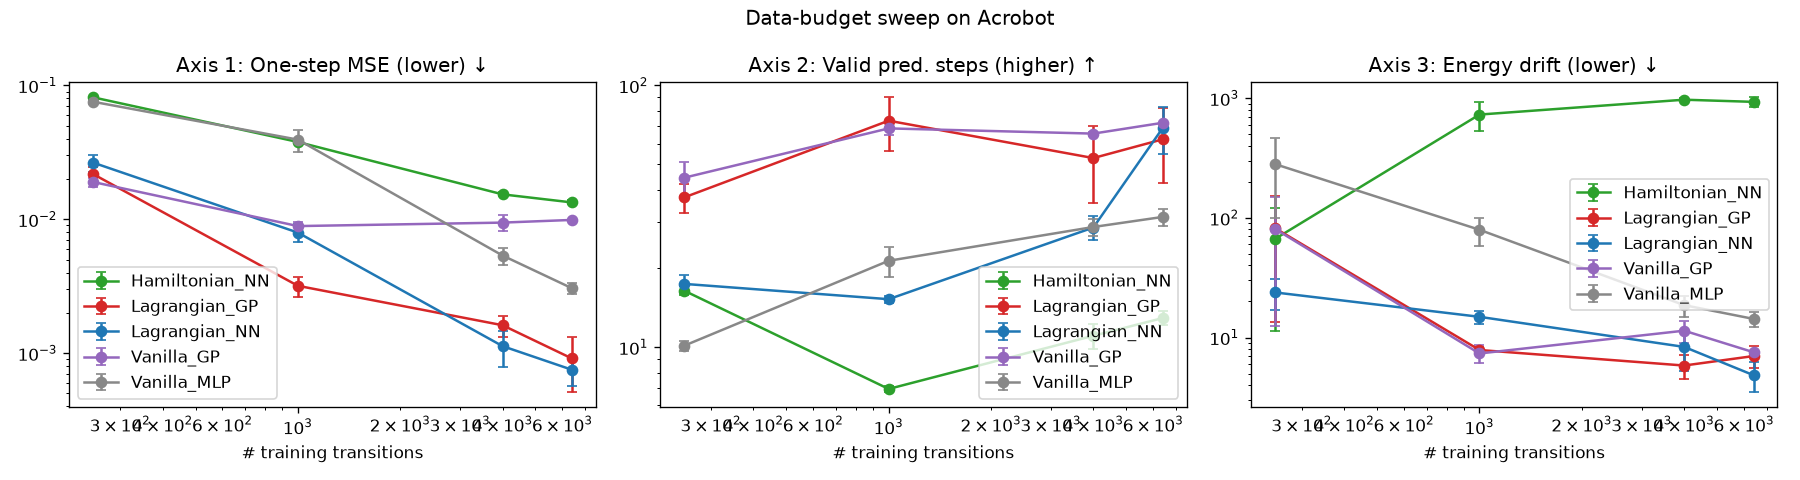
\includegraphics[width=0.49\textwidth]{figures/sweep_Acrobot.png}
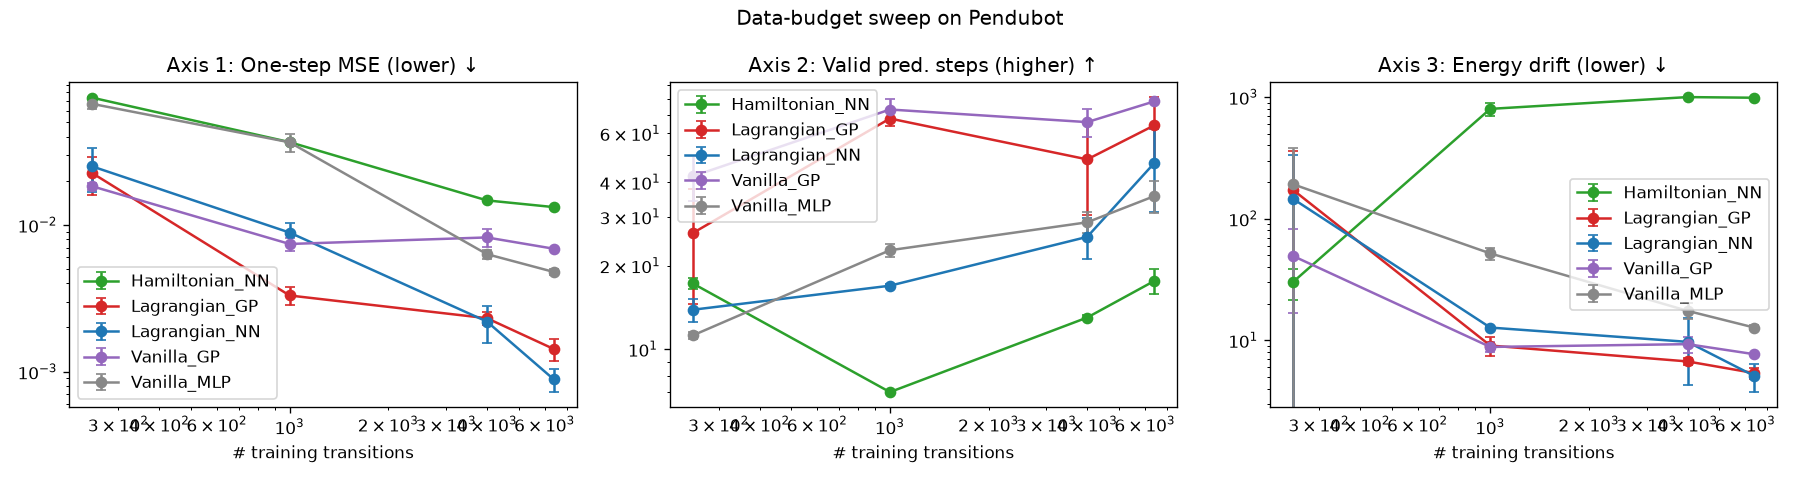
\includegraphics[width=0.49\textwidth]{figures/sweep_Pendubot.png}
\caption{Data-budget sweep on the Acrobot (left) and Pendubot (right). Each
panel shows one dynamics axis versus the number of training transitions
(log--log), averaged over seeds with standard-deviation error bars.}
\label{fig:sweep}
\end{figure*}

\textbf{Accuracy and energy.} The LNN is the most accurate model on both systems
(one-step MSE below $10^{-3}$) and has the lowest energy drift, reflecting its
matched physical structure. The black-box MLP is a competent middle performer.

\textbf{Stability.} On the chaotic free-swing task, the GP yields the
\emph{longest} valid prediction time on both systems---more than twice the
MLP's---despite its larger one-step error. Smoothing toward the GP prior appears
to damp the error growth that destabilises the MLP. The LGP inherits much of this
stability while retaining LNN-level one-step accuracy, giving the best overall
balance: on the Pendubot it even exceeds the plain LNN in valid steps.

\textbf{The wrong prior hurts.} The HNN is the worst model on every dynamics
axis. Its identity-mass assumption is badly violated by the configuration-
dependent inertia of these robots, so it fits poorly even one step ahead and
diverges in $60$--$87\%$ of rollouts (its huge energy-drift values are an
artifact of these divergences). This is a concrete case where an ill-matched
physics prior is worse than no prior at all.

\textbf{Data efficiency} (Fig.~\ref{fig:sweep}). At the smallest budget
($250$ points) the GP and the Lagrangian models are already far more accurate
than the MLP, whose advantage only appears with more data. Physics priors and
GP smoothing both help most exactly when data are scarce.

\subsection{Downstream Swing-Up Control (Axis 4)}
\label{sec:control}
We close the loop with an energy-shaping controller that pumps energy into the
\emph{true} plant using a model's energy estimate,
\begin{equation}
u = k_e\,(E_{\mathrm{top}}-E_{\mathrm{model}}(x))\,\dot q_{\mathrm{act}}
   - k_p\,q_{\mathrm{act}} - k_d\,\dot q_{\mathrm{act}},
\end{equation}
clipped to a torque limit, where $E_{\mathrm{top}}$ is the upright energy under
the same model (so any constant offset cancels) and $q_{\mathrm{act}}$ is the
actuated joint. Only models that expose an energy function---the LNN, HNN, and
LGP---can drive this controller; the black-box MLP and GP cannot, which is itself
a result. We report the normalised tip height reached ($0$ down, $1$ upright)
and the success rate over fixed initial conditions, with a true-energy
\emph{Oracle} as the ceiling (Table~\ref{tab:control}, Fig.~\ref{fig:control}).

\begin{table}[t]
\caption{Energy-based swing-up. Mean normalised tip height and success rate
(seed-averaged). The Oracle uses the true energy. The MLP and GP have no energy
function and cannot drive an energy-based controller (N/A).}
\label{tab:control}
\centering
\begin{tabular}{llcc}
\toprule
System & Model & Mean tip height & Success \\
\midrule
\multirow{4}{*}{Acrobot}
 & Oracle          & $0.97$ & $100\%$ \\
 & Lagrangian NN   & $\mathbf{0.69}$ & $\mathbf{33\%}$ \\
 & Lagrangian GP   & $0.62$ & $25\%$ \\
 & Hamiltonian NN  & $0.50$ & $0\%$ \\
\midrule
\multirow{4}{*}{Pendubot}
 & Oracle          & $0.96$ & $100\%$ \\
 & Lagrangian NN   & $\mathbf{0.84}$ & $\mathbf{50\%}$ \\
 & Hamiltonian NN  & $0.67$ & $8\%$ \\
 & Lagrangian GP   & $0.61$ & $17\%$ \\
\bottomrule
\end{tabular}
\end{table}

\begin{figure}[t]
\centering
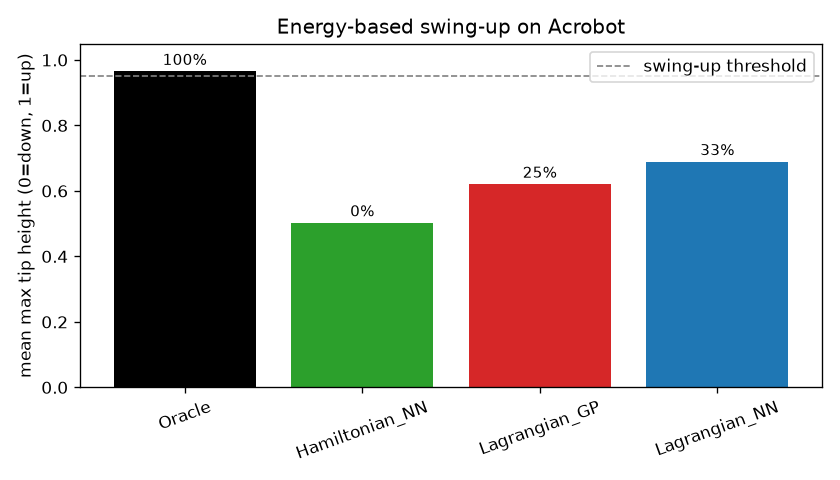
\includegraphics[width=0.49\columnwidth]{figures/control_Acrobot.png}
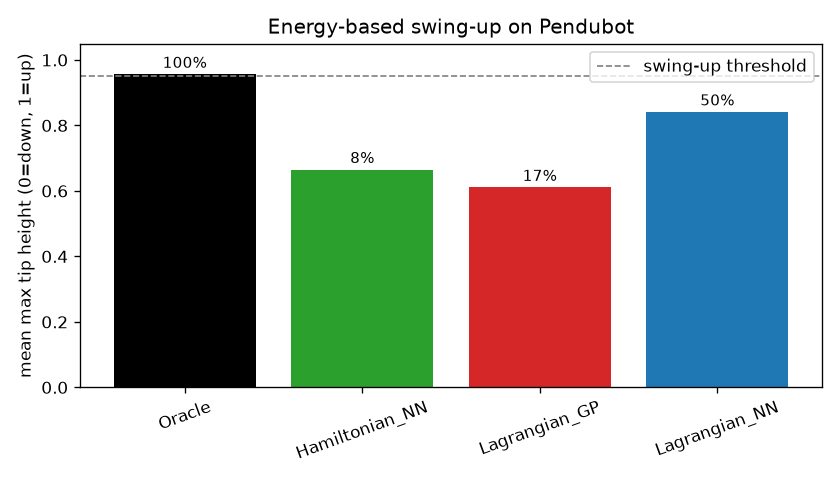
\includegraphics[width=0.49\columnwidth]{figures/control_Pendubot.png}
\caption{Swing-up performance. Bars show mean tip height; the percentage above
each bar is the success rate. Black-box models are absent because they provide no
energy function.}
\label{fig:control}
\end{figure}

The ranking on control follows energy-model quality: the LNN, with the most
accurate learned energy, swings up best among learned models (up to $50\%$
success on the Pendubot), the LGP follows, and the HNN---whose energy is
unreliable---largely fails. No learned model matches the Oracle, underlining that
partial energy errors still cost control performance. This directly connects
predictive quality to downstream usefulness.

\section{Discussion: A Map of When Physics Priors Help}
Taken together, the four axes yield a consistent picture.
\emph{First}, physics priors help most when their structure matches the system:
the LNN's learned positive-definite, configuration-dependent mass matrix is the
single most valuable ingredient here, driving its wins on accuracy, energy, and
control. \emph{Second}, an ill-matched prior can be actively harmful---the HNN's
identity-mass assumption makes it worse than a black box and unstable.
\emph{Third}, the benefit of any prior is largest in the low-data regime and on
long-horizon, energy-sensitive tasks; at high data with only one-step accuracy in
view, the black-box MLP is competitive. \emph{Fourth}, uncertainty-aware models
(GPs) buy rollout stability and data efficiency that are complementary to
hard structural priors, and combining the two (the LGP) gives the best balance on
the dynamics axes. No single model wins everything, which is precisely the
practical guidance a practitioner needs.

\section{Limitations and Future Work}
Our study is in simulation on two planar systems with a single, simple
energy-shaping controller; absolute swing-up success is modest because the
learned energy is imperfect and the controller is not re-tuned per model. The
exact GP is capped in training-set size, and the GP shows little seed variance at
the largest budget because its fit is deterministic there. Natural extensions
include observation and process noise, per-model controller tuning or an
LQR catch near the top, model-predictive control so that black-box models can
also be evaluated downstream, additional systems (e.g.\ cart-pole), and sparse or
deep-kernel GPs to scale the GP and LGP to larger budgets.

\section{Conclusion}
We presented a controlled, reproducible benchmark of five dynamics models on two
underactuated systems across four evaluation axes. Rather than crowning a single
method, our results map out \emph{when} physics priors help: most when the prior
matches the system's structure, when data are scarce, and on long-horizon,
energy-sensitive tasks---while a mismatched prior can be worse than none. We hope
the released pipeline serves as a reusable testbed for physics-informed dynamics
learning.

\section*{Reproducibility}
Code, configurations, datasets, and the scripts that regenerate every table and
figure are available at
\url{https://github.com/amirhossein-fattahi/piml-underactuated}.

\begin{thebibliography}{99}
\bibitem{karniadakis2021} G.~E. Karniadakis \emph{et al.}, ``Physics-informed
machine learning,'' \emph{Nature Reviews Physics}, vol.~3, pp.~422--440, 2021.
\bibitem{raissi2019} M.~Raissi, P.~Perdikaris, and G.~E. Karniadakis,
``Physics-informed neural networks,'' \emph{Journal of Computational Physics},
vol.~378, pp.~686--707, 2019.
\bibitem{lutter2019} M.~Lutter, C.~Ritter, and J.~Peters, ``Deep Lagrangian
Networks: Using physics as model prior for deep learning,'' in \emph{ICLR},
2019.
\bibitem{cranmer2020} M.~Cranmer \emph{et al.}, ``Lagrangian Neural Networks,''
in \emph{ICLR Workshop on Integration of Deep Neural Models and Differential
Equations}, 2020.
\bibitem{greydanus2019} S.~Greydanus, M.~Dzamba, and J.~Yosinski, ``Hamiltonian
Neural Networks,'' in \emph{NeurIPS}, 2019.
\bibitem{zhong2020} Y.~D. Zhong, B.~Dey, and A.~Chakraborty, ``Symplectic
ODE-Net: Learning Hamiltonian dynamics with control,'' in \emph{ICLR}, 2020.
\bibitem{saemundsson2020} S.~S\ae mundsson, A.~Terenin, K.~Hofmann, and M.~P.
Deisenroth, ``Variational integrator networks for physically structured
embeddings,'' in \emph{AISTATS}, 2020.
\bibitem{rasmussen2006} C.~E. Rasmussen and C.~K.~I. Williams, \emph{Gaussian
Processes for Machine Learning}. MIT Press, 2006.
\bibitem{nguyen2011} D.~Nguyen-Tuong and J.~Peters, ``Model learning for robot
control: a survey,'' \emph{Cognitive Processing}, vol.~12, no.~4,
pp.~319--340, 2011.
\bibitem{deisenroth2011} M.~P. Deisenroth and C.~E. Rasmussen, ``PILCO: A
model-based and data-efficient approach to policy search,'' in \emph{ICML},
2011.
\bibitem{spong1995} M.~W. Spong, ``The swing up control problem for the
Acrobot,'' \emph{IEEE Control Systems Magazine}, vol.~15, no.~1, pp.~49--55,
1995.
\bibitem{tedrake} R.~Tedrake, \emph{Underactuated Robotics: Algorithms for
Walking, Running, Swimming, Flying, and Manipulation}. Course notes, MIT, 2023.
\end{thebibliography}

\end{document}
